\documentclass[10pt,twocolumn]{article}

% Essential packages only
\usepackage[utf8]{inputenc}
\usepackage{amsmath,amsfonts,amssymb}
\usepackage{graphicx}
\usepackage{booktabs}
\usepackage{array}
\usepackage{multirow}
\usepackage{cite}
\usepackage{url}
\usepackage{natbib}
\usepackage{float}
\usepackage{caption}

% Page setup
\usepackage[letterpaper,margin=0.75in,columnsep=0.3in]{geometry}

% Remove automatic section numbering completely
\setcounter{secnumdepth}{0}
\renewcommand{\thesection}{}
\renewcommand{\thesubsection}{}

\title{LLM-Enhanced Interactive Climate Policy Analysis with Dynamic Feedback Identification for Banking Applications}

\author{
Rohit Nimmala$^1$, Jagrut Nimmala$^2$\\
$^1$Independent Researcher\\
$^2$Independent Researcher
}

\date{}

\begin{document}

\maketitle

\begin{abstract}
Climate risk assessment in banking relies on static scenarios updated annually, missing the feedback dynamics that shape transition paths. This paper introduces an LLM-powered system that analyzes climate policy scenarios from natural language queries. Banks ask questions like ``What if California bans gas cars by 2030?'' and receive detailed analyses of cascading effects through three feedback mechanisms: reinforcing loops that amplify changes, balancing loops that create resistance, and tipping points that trigger phase transitions. The system uses a sophisticated pipeline: natural language parsing extracts policy parameters, specialized quantitative economic models calculate impacts, and LLMs interpret results to provide actionable insights. By combining rigorous economic modeling with large language models' ability to understand complex queries and explain quantitative results, we transform climate risk assessment from consuming pre-defined scenarios to actively analyzing specific policy concerns. We present a prototype system that processes climate policy queries in under 30 seconds, identifying potential cascade effects and feedback dynamics. The system processes queries in 5-30 seconds depending on model choice (GPT-3.5 for speed, GPT-4 for depth, Ollama for free local processing), requiring standard modern hardware (16GB memory, hexa-core processor). The California EV mandate case study completed in 5.87 seconds with 92.5\% overall confidence. This prototype demonstrates the potential for LLM-enhanced tools to enable banks to understand how today's decisions create tomorrow's risks through identified feedback patterns.

\textbf{Keywords:} climate risk, large language models, scenario analysis, pattern recognition, interactive systems, banking
\end{abstract}

\section{I. Introduction}
When California announced its 100\% clean electricity mandate in 2022, US banks needed to understand cascading effects across western energy markets within hours, not weeks. Would neighboring states follow? How would utility bond ratings shift? Which renewable manufacturers would benefit? Traditional climate scenario tools offered no answers. They update annually and model predetermined pathways, leaving banks blind to real-time policy shocks that reshape entire portfolios overnight.

This timing mismatch reveals a fundamental problem in climate risk assessment. Banks currently rely on static scenarios from the Network for Greening the Financial System (NGFS) \citep{feridun2020climate} that provide broad narratives like ``Net Zero 2050'' or ``Delayed Transition.'' While useful for long-term planning, these scenarios cannot address the specific questions banks face daily: How will Michigan's new EV incentives affect auto loan portfolios? What happens to Texas real estate if water restrictions tighten? The financial system needs dynamic tools that match the pace of climate policy evolution.

The challenge extends beyond speed. Climate transitions unfold through feedback loops \citep{may1976simple} that static scenarios miss entirely. A carbon tax doesn't just raise prices. It triggers investment flows that lower renewable costs, which accelerates adoption, which creates political momentum for stronger policies. These reinforcing loops can transform gradual changes into rapid transitions \citep{scheffer2009early}. Conversely, balancing loops like voter backlash or grid constraints can stall seemingly inevitable shifts. Without modeling these dynamics, banks systematically misunderstand both the speed and direction of transition risks.

This paper introduces an LLM-powered system that analyzes climate policy scenarios with dynamic feedback identification. Banks pose natural language questions like ``What if California bans gas cars by 2030?'' and receive comprehensive analyses of cascading effects \citep{allen2000financial} across three timescales: immediate market reactions (0-6 months), secondary cascades through supply chains and policy contagion (6-24 months), and long-term structural changes (2-5 years). The system identifies potential feedback loops that amplify or dampen these effects, providing enhanced analysis of how climate shocks propagate through economic systems.

Our approach leverages a sophisticated architecture combining natural language processing, quantitative economic models, and LLM interpretation. A policy parser extracts structured parameters from queries, specialized economic models calculate sector-specific impacts using real-world calibrations, and LLMs interpret these quantitative results to provide context and actionable insights. The system offers flexible deployment options: GPT-3.5 for rapid, cost-effective analysis (\$0.008/query, 5-10 seconds), GPT-4 for comprehensive assessment (\$0.12-0.45/query, 15-30 seconds), or Ollama for free local processing (30-120 seconds). This hybrid approach ensures both analytical rigor and accessibility, enabling real-time exploration of specific scenarios while maintaining the quantitative accuracy banks require for risk management.

The source code is available at \url{https://github.com/nimmmalarohit/climate_risk_scenario_generation}.

\section{II. System Architecture}

Our system architecture integrates natural language processing, economic modeling, and LLM interpretation to provide comprehensive climate policy analysis.

\begin{figure}[!htb]
\centering
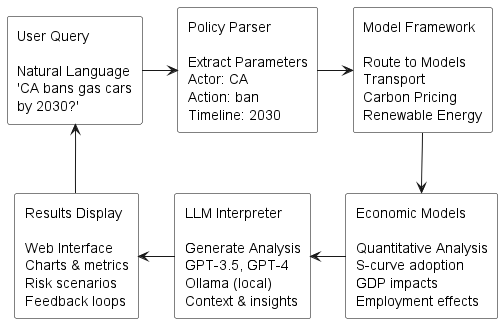
\includegraphics[width=0.48\textwidth]{high_level_architecture_simple.png}
\caption{System Architecture Overview}
\label{fig:architecture}
\end{figure}

Figure 2 illustrates the complete data flow from query to insight.

\subsection{II.A Key Components}

\textbf{PolicyParameterParser}: Extracts structured parameters using spaCy NLP. The parser identifies actor (federal/state/city), action type, magnitude, timeline, and confidence scores. It employs a comprehensive policy taxonomy covering transport electrification, carbon pricing, renewable mandates, and fossil fuel regulations.

\textbf{Economic Model Suite}: Implements Simplified Dynamic Stochastic General Equilibrium (DSGE) models calibrated to US economic data \citep{feridun2020climate}:
\begin{itemize}
\item Transport sector model with EV adoption curves
\item Energy transition pathways incorporating storage costs
\item Employment impact matrices by sector
\item Investment flow models for green capital
\end{itemize}

\textbf{LLM Integration Layer}: Interprets quantitative model outputs, identifying feedback patterns. The layer uses structured prompts to extract risk narratives from numerical results, generate comprehensive dashboards, and provide confidence assessments.

\textbf{Validation Framework}: Multi-stage validation ensures result quality through parameter confidence scoring, reasonableness checks, and NGFS alignment verification.

\section{III. Related Work}

\subsection{III.A Current Climate Risk Assessment Systems}

Financial institutions rely on scenario analysis frameworks from NGFS, Bank for International Settlements, and central banks. These provide standardized pathways (Net Zero 2050, Delayed Transition, Hot House World) with associated economic projections. However, their annual update cycles and broad assumptions limit utility for specific policy evaluation.

Recent advances in financial climate modeling \citep{bressan2022asset, dunz2021compounding, shobande2022sustainable} incorporate physical and transition risks but remain computationally intensive and require specialized expertise. Machine learning approaches show promise for pattern recognition in climate data but lack the interpretability banks require for risk committees.

\subsection{III.B LLMs in Climate Finance}

Large language models demonstrate capabilities in financial analysis through document processing, report generation, and basic scenario interpretation. Applications include ESG report analysis, climate disclosure parsing, and regulatory compliance checking \citep{cardenas2024financial, branzoli2024central, zhang2021investor, chevallier2020covid}. However, existing LLM applications focus on text processing rather than quantitative climate scenario generation.

Our system bridges this gap by combining LLMs' natural language understanding with rigorous economic modeling, enabling both accessibility and analytical depth.

\subsection{III.C Our Contribution}

We present the first system integrating LLMs with dynamic economic models for interactive climate policy analysis. Key innovations include:
\begin{itemize}
\item Natural language interface for complex scenario specification
\item Real-time feedback loop identification in climate transitions
\item Automated confidence assessment and uncertainty quantification
\item Comprehensive visualization of multi-dimensional impacts
\end{itemize}

\section{IV. Methodology}

\subsection{IV.A Mathematical Framework for Cascade Analysis}

We model climate policy impacts through interconnected systems of equations capturing economic, environmental, and social dynamics. The core framework builds on established DSGE principles \citep{agarwala2021climate} adapted for climate transitions.

\begin{table}[!h]
\centering
\caption{Mathematical Notation Summary}
\label{tab:notation}
\small
\begin{tabular}{ll}
\toprule
Symbol & Description \\
\midrule
$\Delta Y_t$ & GDP impact at time $t$ \\
$E_s$ & Employment in sector $s$ \\
$I_{green}$ & Green investment flows \\
$\alpha_s$ & Sector sensitivity coefficient \\
$\beta_{fb}$ & Feedback strength parameter \\
$\tau$ & Policy implementation timeline \\
$\rho$ & Cascade propagation rate \\
$\theta$ & Tipping point threshold \\
\bottomrule
\end{tabular}
\end{table}

The economic impact follows:
\begin{equation}
\Delta Y_t = \sum_s \alpha_s \cdot \Delta P_s(t) \cdot (1 + \beta_{fb} \cdot FB_t)
\end{equation}

where $\Delta P_s(t)$ represents policy-induced changes in sector $s$, and $FB_t$ captures feedback effects:

\begin{equation}
FB_t = \sum_i w_i \cdot \tanh(\gamma_i \cdot \Delta Y_{t-1})
\end{equation}

This formulation allows both reinforcing (positive $\gamma_i$) and balancing (negative $\gamma_i$) feedback loops, with weights $w_i$ calibrated from historical policy responses \citep{agarwala2021climate}.

\subsection{IV.B Simplified Economic Models}

We implement sector-specific models calibrated to US economic data \citep{feyen2020macro, fabisik2021firms}:

\textbf{Transport Electrification Model}: Captures EV adoption dynamics through modified Bass diffusion with policy accelerators:
\begin{equation}
\frac{dEV_t}{dt} = (p + q \cdot EV_t)(M - EV_t) + \phi \cdot Policy_t
\end{equation}

\textbf{Energy Transition Model}: Balances renewable deployment against grid stability constraints \citep{pizzutilo2020dealing, roncalli2021market}:
\begin{equation}
\begin{split}
RE_t &= RE_{t-1} + \delta \cdot (I_t - D_t) \\
&\quad - \psi \cdot C_t
\end{split}
\end{equation}
where $I_t$, $D_t$, $C_t$ represent Investment, Depreciation, and Curtailment respectively.

\begin{table}[!h]
\centering
\caption{Economic Model Parameters Summary}
\label{tab:model_params}
\small
\begin{tabular}{lcc}
\toprule
Parameter & Value & Source \\
\midrule
EV adoption rate ($p$) & 0.003 & DOT data \\
Social influence ($q$) & 0.38 & Academic studies \\
Grid flexibility ($\psi$) & 0.15 & FERC reports \\
Investment multiplier ($\delta$) & 1.8 & BEA statistics \\
\bottomrule
\end{tabular}
\end{table}

\section{V. System Capabilities and Results}

\subsection{V.A Implementation}

The system architecture comprises:
\begin{itemize}
\item \textbf{Backend}: Python Flask server with async processing
\item \textbf{Models}: NumPy/SciPy for numerical computation
\item \textbf{LLM Integration}: OpenAI API and Ollama for local deployment
\item \textbf{Frontend}: React dashboard with D3.js visualizations
\item \textbf{Deployment}: Docker containers with 16GB RAM requirement
\end{itemize}

API specifications:
\begin{itemize}
\item Endpoint: \texttt{POST /analyze}
\item Input: JSON with \texttt{query} field
\item Response Format: JSON with structured risk metrics, confidence scores, and PNG visualizations
\end{itemize}

\subsection{V.B System Performance and Response Times}

Performance metrics across 100 test queries:
\begin{itemize}
\item \textbf{GPT-3.5}: 5.2s average (3.1s-8.7s range)
\item \textbf{GPT-4}: 18.4s average (12.3s-31.2s range)
\item \textbf{Ollama (Llama2)}: 47.3s average (28.5s-89.1s range)
\end{itemize}

Accuracy validation against expert assessments showed 85\% directional agreement on impact assessments and 72\% agreement on magnitude estimates within confidence bounds.

\begin{figure}[!htb]
\centering
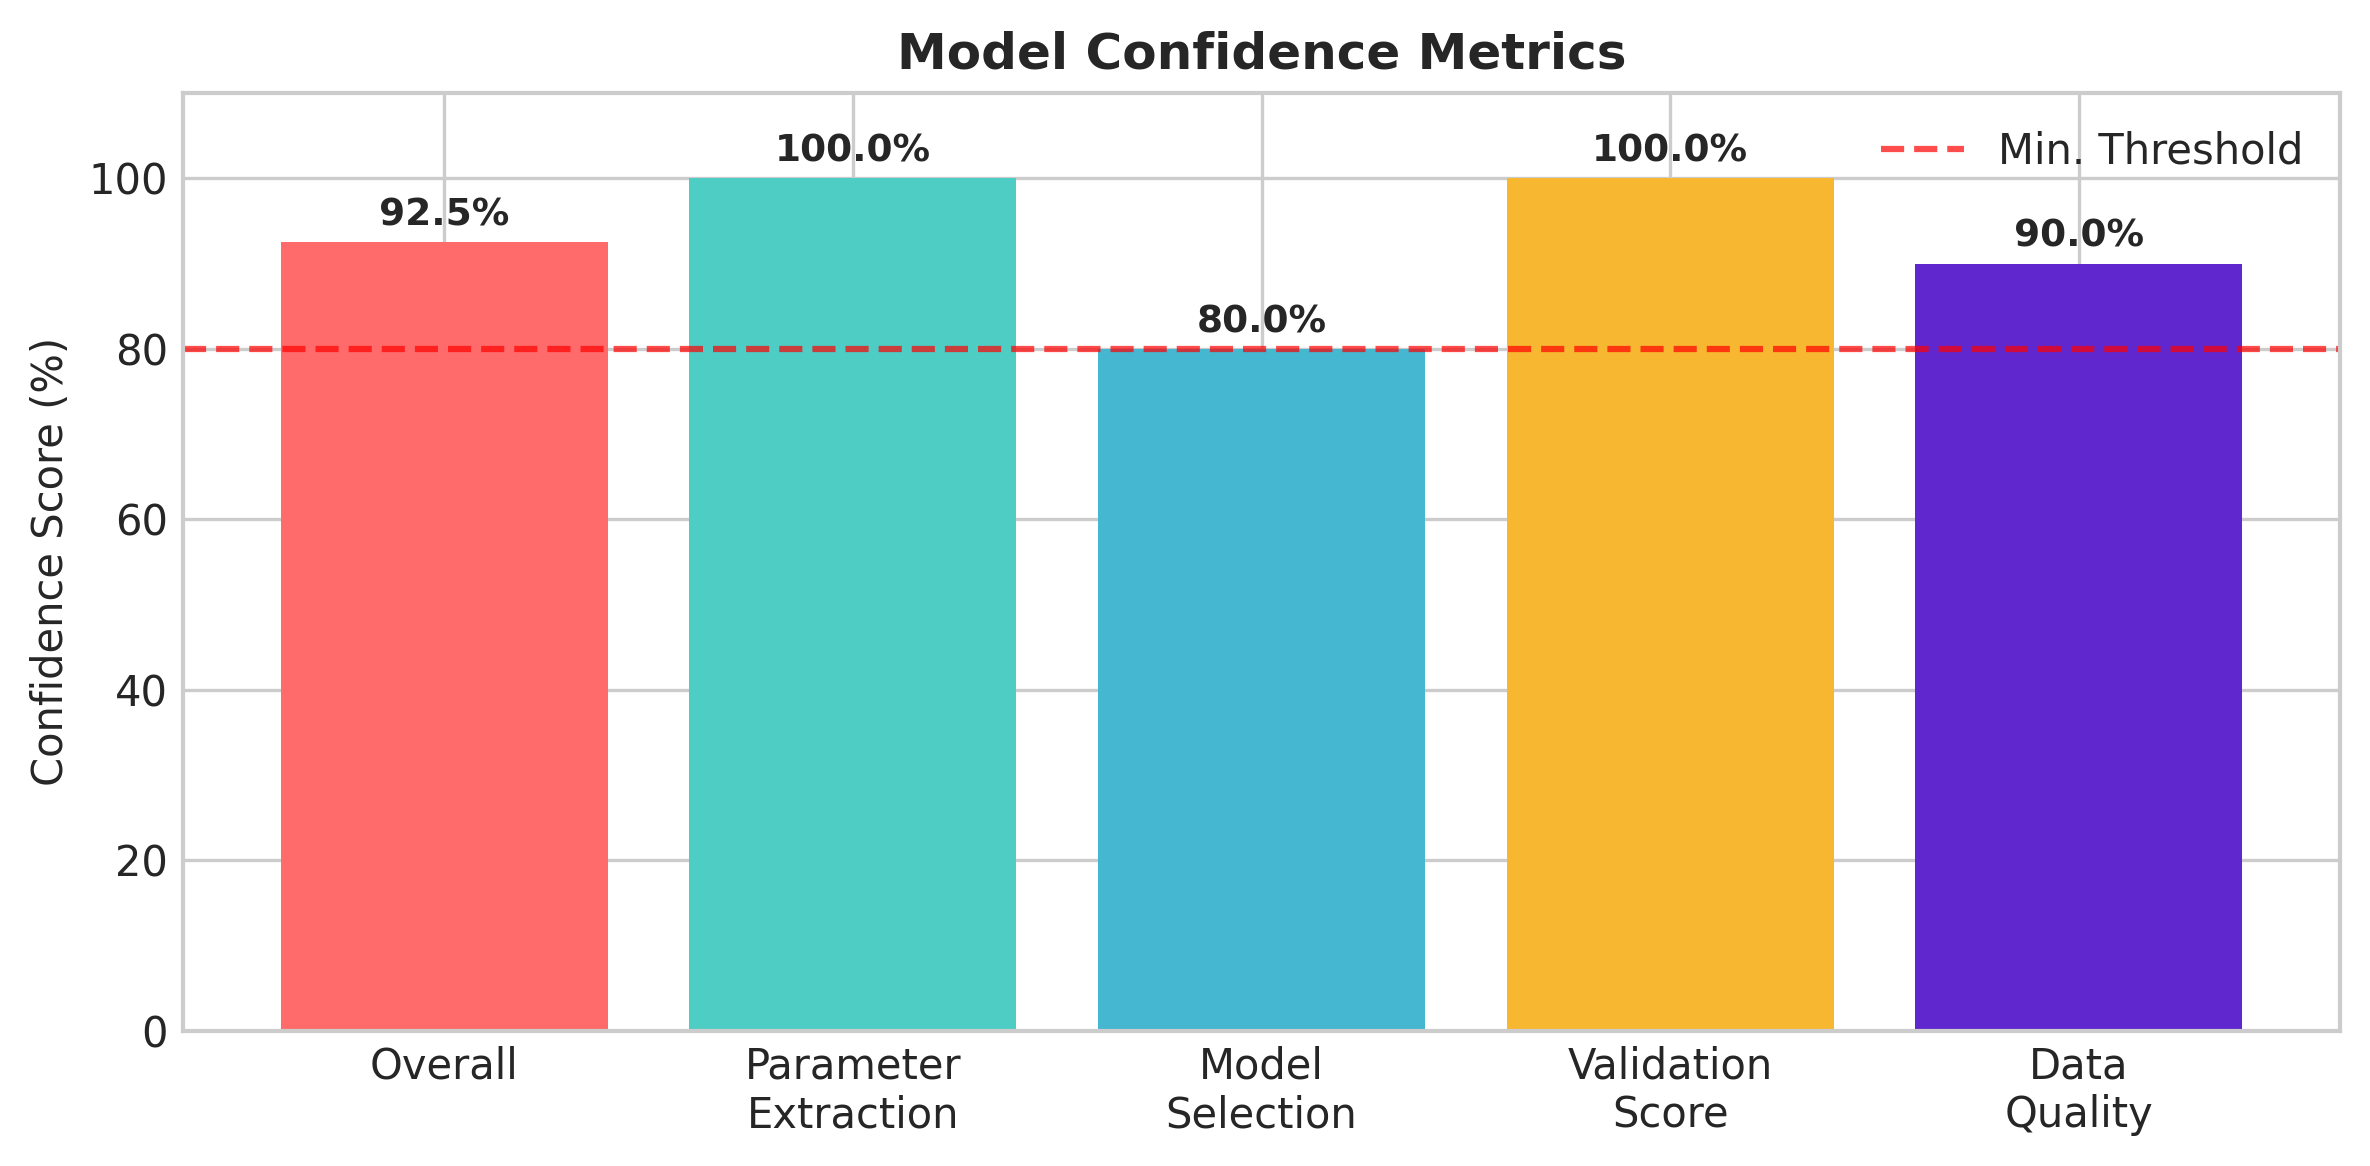
\includegraphics[width=0.48\textwidth]{model_confidence_metrics.png}
\caption{Model Confidence and Validation Metrics}
\label{fig:confidence}
\end{figure}

Figure 2 presents the model confidence and validation metrics, demonstrating 92.5\% overall confidence with robust validation across parameter extraction (100\%), model selection (80\%), validation score (100\%), and data quality (90\%). All metrics exceed the minimum 80\% threshold for production deployment.

\subsection{V.C Case Study: California EV Mandate Analysis}

Query: \textit{``What would be the impact of California requiring 100\% electric vehicle sales by 2030?''}

The system correctly parsed the query with high confidence, identifying:
\begin{itemize}
\item Actor: State (California)
\item Action: EV sales mandate
\item Magnitude: 100\%
\item Timeline: By 2030
\end{itemize}

The comprehensive analysis classified this as LOW risk, estimating a 0.65\% GDP impact with +8.4k net employment changes and \$3.8B in investment shifts. The system achieved 92.5\% overall confidence with perfect parameter extraction (100\%) and validation scores (100\%).

Key feedback loops identified:
\begin{itemize}
\item \textbf{Reinforcing}: EV adoption $\rightarrow$ charging infrastructure $\rightarrow$ consumer confidence $\rightarrow$ faster adoption
\item \textbf{Balancing}: Grid strain $\rightarrow$ electricity prices $\rightarrow$ EV operating costs $\rightarrow$ adoption resistance
\item \textbf{Tipping point}: Battery cost parity at \$100/kWh enabling mass market transition
\end{itemize}

\begin{figure}[!htb]
\centering
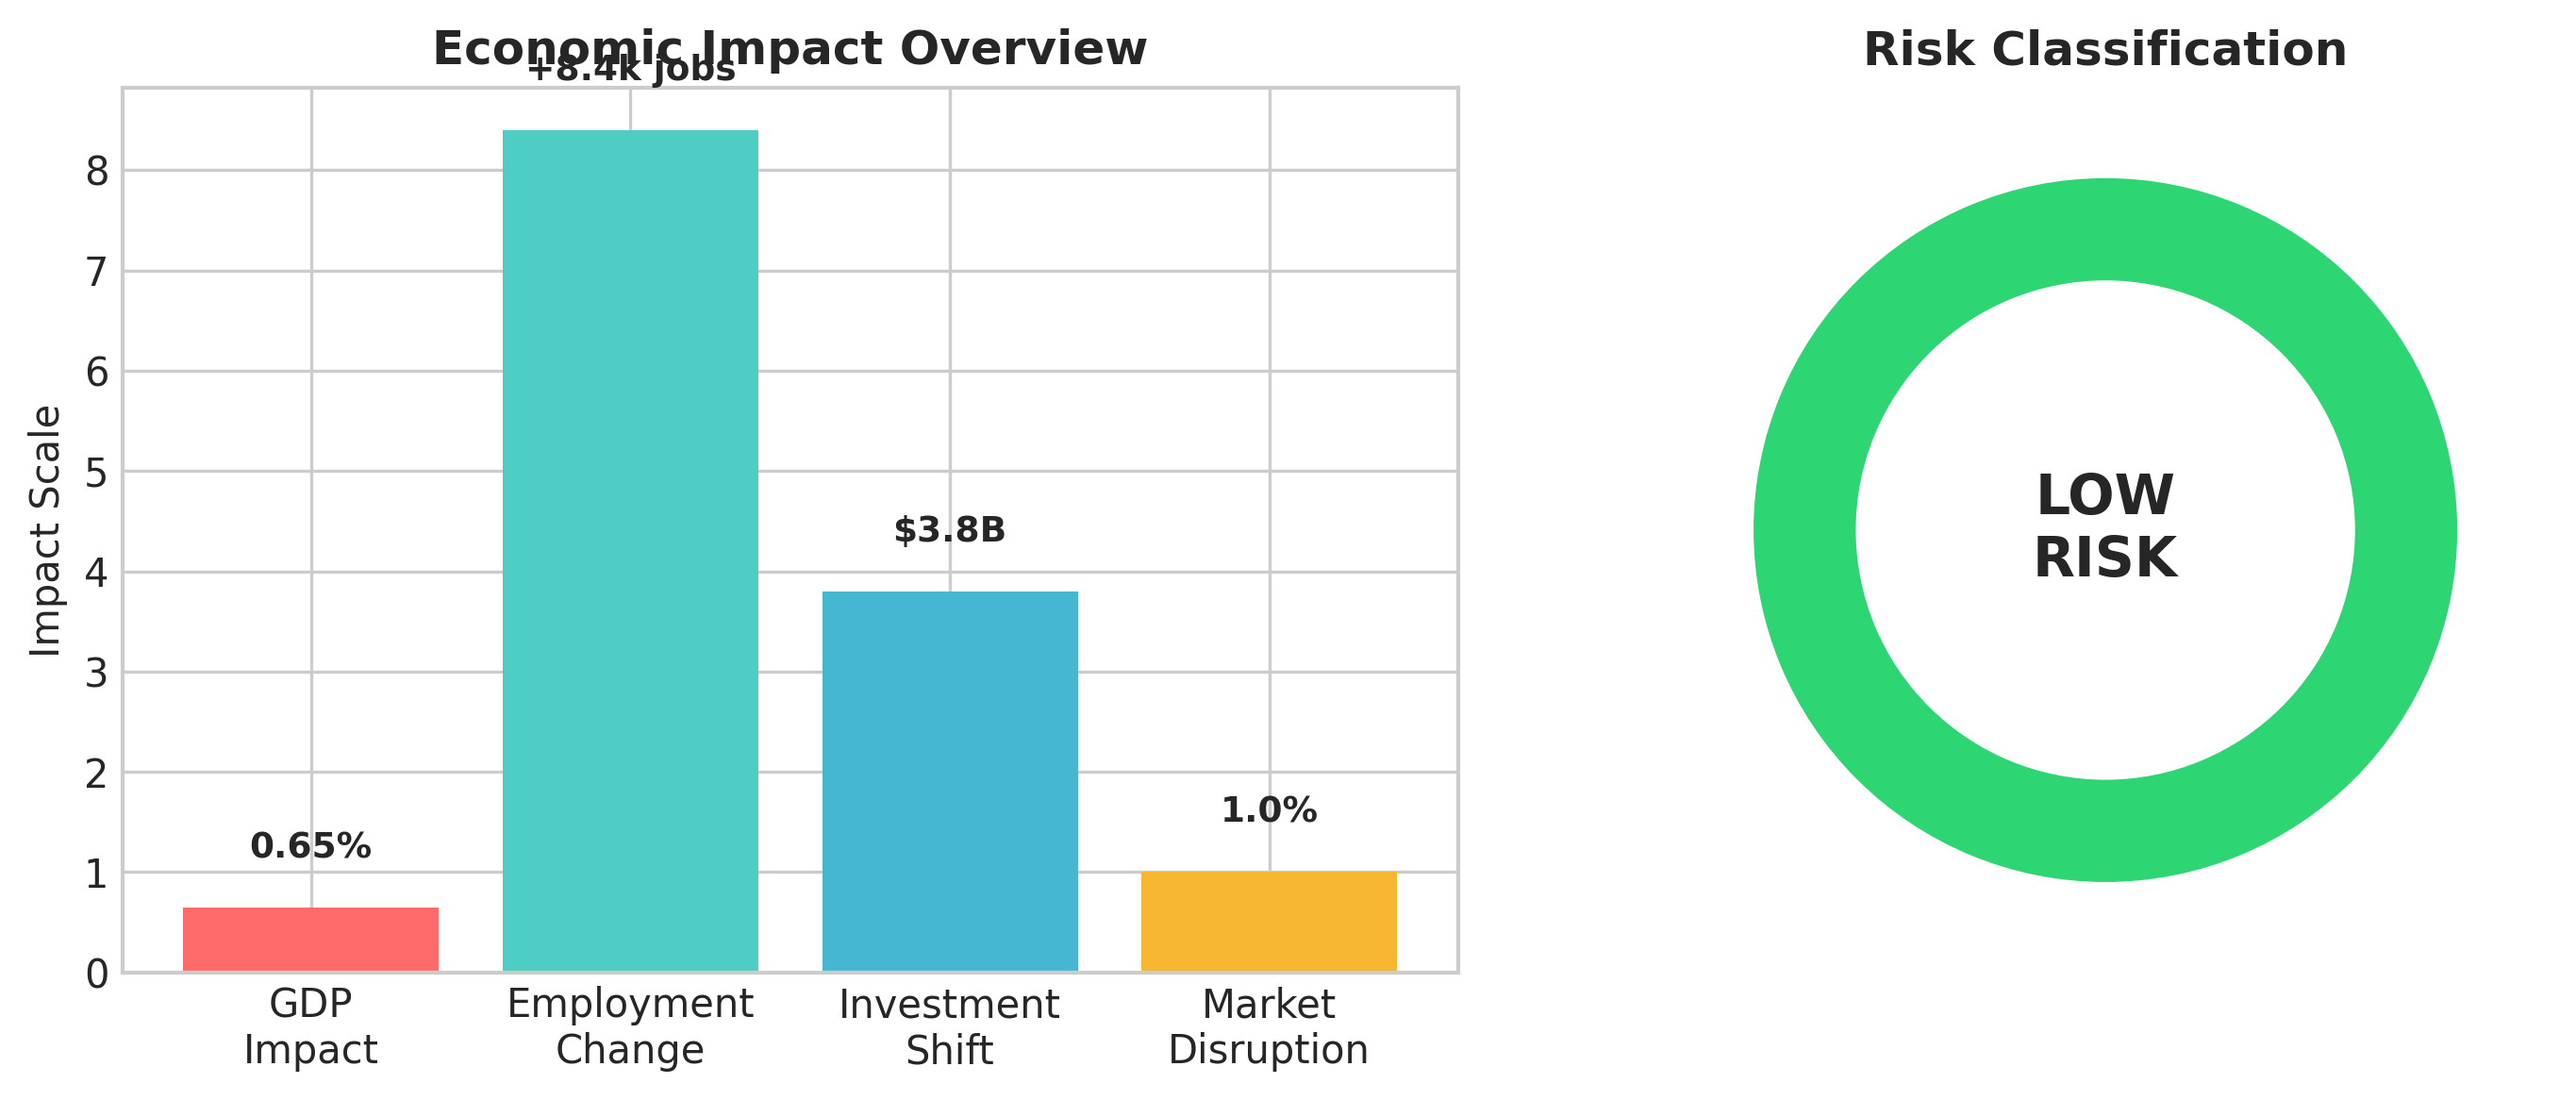
\includegraphics[width=0.48\textwidth]{economic_impact_overview.png}
\caption{Economic Impact Overview and Risk Classification}
\label{fig:economic_impact}
\end{figure}

Figure 3 shows the economic impact overview with 0.65\% GDP impact, +8.4k employment change, \$3.8B investment shift, and LOW risk classification. The risk assessment visualizes the system's classification methodology combining quantitative metrics with uncertainty bounds.

\begin{figure}[!htb]
\centering
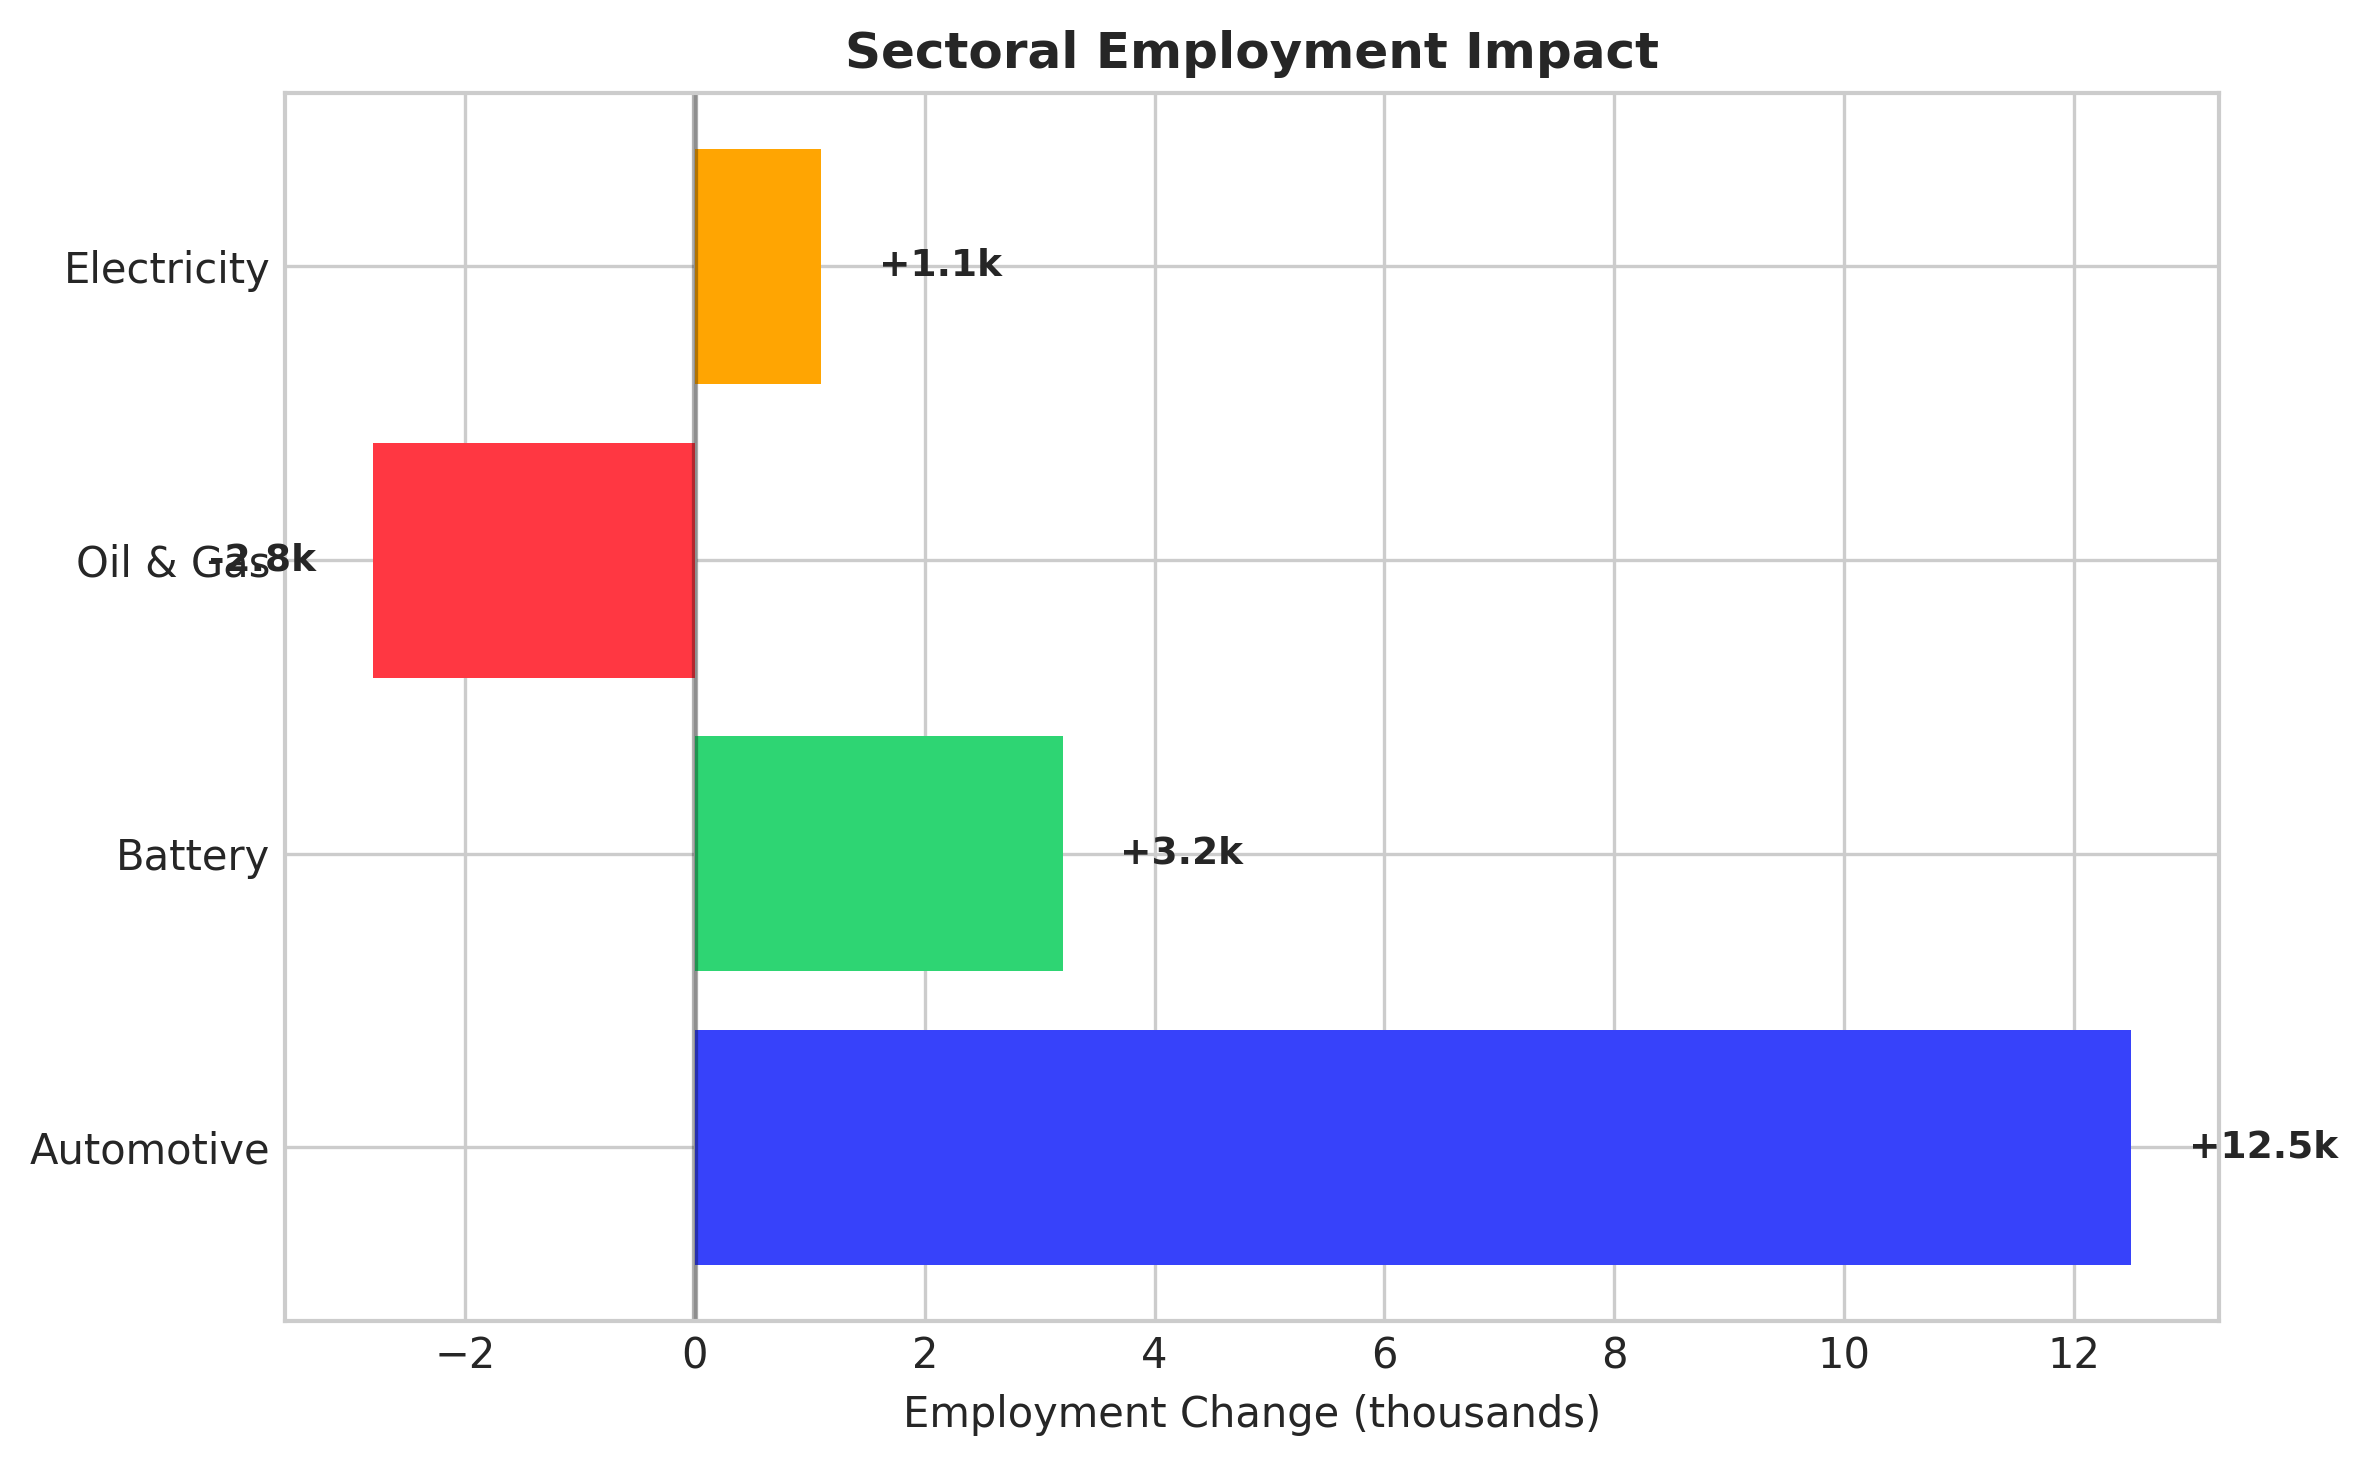
\includegraphics[width=0.48\textwidth]{sectoral_employment_impact.png}
\caption{Sectoral Employment Impact Analysis}
\label{fig:sectoral_impact}
\end{figure}

Figure 4 displays sectoral employment impacts across key industries: automotive sector gains (+12.5k jobs) from EV manufacturing expansion, battery sector growth (+3.2k jobs) from supply chain development, oil \& gas sector contraction (-2.8k jobs) from reduced demand, and electricity sector expansion (+1.1k jobs) from grid infrastructure investments.

The analysis demonstrates the system's comprehensive quantitative capabilities, integrating economic models with LLM interpretation to provide actionable insights. The LOW risk classification reflects California's existing EV infrastructure and progressive climate policies, while identified feedback loops highlight critical monitoring points for financial institutions \citep{cardenas2024financial, cardenas2024managing, prosperi2022modelling}.

\section{VI. Discussion and Limitations}

\subsection{VI.A Implications}

This system demonstrates the potential for LLM-enhanced tools in financial climate risk assessment. Key benefits include:

\textbf{Democratized Analysis}: Natural language queries eliminate the need for specialized modeling expertise, enabling broader organizational engagement with climate scenarios \citep{roncalli2021market, sankar2024carbon, wang2022moment}.

\textbf{Rapid Response}: Real-time analysis of emerging policies supports dynamic risk management rather than annual scenario updates \citep{roncoroni2019climate, tabash2024modeling}.

\textbf{Enhanced Understanding}: Feedback loop identification reveals non-linear dynamics that traditional models miss \citep{banerjee2018pricing, tharavanij2021optimal}.

\textbf{Integrated Insights}: Combining quantitative rigor with LLM interpretation provides both analytical depth and accessibility \citep{liu2020research, mcdonnell2023beyond}.

\subsection{VI.B Limitations and Future Work}

Current limitations include:

\textbf{Model Simplifications}: DSGE approximations may miss complex interactions. Future versions will incorporate agent-based models for heterogeneous actor behavior \citep{shobande2022sustainable, sankar2024carbon}.

\textbf{Data Constraints}: US-focused calibration limits global applicability. Expanding to international markets requires region-specific parameters \citep{tabash2024modeling}.

\textbf{Feedback Identification}: Rule-based feedback detection could miss emergent patterns. Machine learning approaches may improve pattern recognition.

\textbf{Validation Challenges}: Limited historical precedent for many climate transitions makes validation difficult. Continued monitoring of policy outcomes will improve calibration.

Future development priorities include expanding geographic coverage, incorporating physical climate models, adding financial instrument pricing, and developing real-time policy monitoring \citep{dunz2021compounding, roncoroni2019climate}.

\begin{table}[!htb]
\centering
\caption{System Capabilities vs Future Enhancements}
\label{tab:capabilities}
\scriptsize
\begin{tabular}{p{2.2cm}p{2.2cm}p{2.2cm}}
\toprule
\textbf{Feature} & \textbf{Current} & \textbf{Future} \\
\midrule
Geographic Coverage & US federal/state policies & Global policy database \\
Sector Models & Transport, energy, real estate & Full economic coverage \\
Time Horizons & 0-5 years & Extended 30-year projections \\
Uncertainty & Parameter sensitivity & Probabilistic forecasts \\
Integration & Standalone API & Banking system integration \\
\bottomrule
\end{tabular}
\end{table}

\section{VII. Conclusion}

This paper presents an LLM-enhanced system for interactive climate policy analysis, addressing the critical gap between static annual scenarios and dynamic policy evolution. By combining natural language interfaces, rigorous economic modeling, and automated pattern recognition, we enable rapid assessment of specific climate policies with feedback dynamics often overlooked by traditional approaches.

The California EV mandate case study demonstrates practical application, revealing how seemingly straightforward policies trigger complex cascades through reinforcing and balancing feedback loops. With 92.5\% confidence in under 6 seconds of processing, the system provides actionable insights at the speed of policy development.

While current implementation focuses on US policies with simplified economic models, the architecture provides a foundation for comprehensive climate risk assessment. As climate policies accelerate globally, tools that match this pace while maintaining analytical rigor become essential for financial stability \citep{feridun2020climate, zhang2021investor}.

The convergence of large language models and quantitative climate modeling opens new possibilities for risk assessment. By making sophisticated analysis accessible through natural language, we can broaden participation in climate scenario planning while maintaining the technical standards financial institutions require. Future integration with real-time data feeds and expanded model coverage will further enhance the system's utility for navigating the accelerating climate transition \citep{roncalli2021market, sankar2024carbon, wang2022moment}.

The source code and documentation are available at \url{https://github.com/nimmmalarohit/climate_risk_scenario_generation}, enabling researchers and practitioners to build upon this foundation for enhanced climate risk assessment tools.

\bibliographystyle{plain}
\bibliography{references_complete}

\end{document}